\subsection{Euler-Lagrange Equation}

\subsubsection{Differential Equation from Physics}

A lot of physical science and engineering is about finding a reduction from a physical problem to differential equations. The newtownian way is to zoom into some local point of the system and derive a set of constraint that holds in the neighborhood. In the case of the vibration of a string, for example, we would find some local segment of string and analyze the tension that acts on it:
\begin{equation}
T(\sin(\theta_1)-\sin(\theta_2)) = m\frac{\partial^2 u}{\partial t^2}
\end{equation}
where $u$ is the vertical displacement from equilibrium. We then take the calculus limit and find out that locally the accelearation of the vertical displacement should be proportional to the curvature. Hence the one-dimensional wave equation:
\begin{equation}
\frac{\partial^2 u}{\partial t^2}=a^2 \frac{\partial^2 u}{\partial x^2}
\end{equation}
\footnote{Here $a$ is a physical parameter intrinsic to the string, i.e., $\sqrt{T}{\rho}$ where $T$ is the tension at equilibrium adn $\rho$ is the density.}

The Lagrangian way is the opposite, we recognize some global objective the system need to be optimized toward, i.e., minimizing the lagragian $L=T -V$ where $T$ is \textit{kinetic energy} and $V$ is \textit{potential energy}. Then, by introduce some perturbation, we extract a constraint which also manifest itself as a differential equation. The following sections descirbes this process in detail.

\begin{framed}
\textbf{Newtonian and Lagrangian Mechanics}\\
\begin{itemize}
\item Newtonian mechanics compute the balance of forces locally and obtain differential equation through

\begin{equation}
F=m\frac{d^2\mathbf{x}}{dt^2}
\end{equation}


\item Lagrangian mechanics translate the physics into some global optimization problem  and reduce to differential equation through the Euler-Lagrange equation

\begin{equation}
\frac{\partial L}{\partial y}- \frac{d}{dx}\frac{\partial L}{\partial y'}=0
\end{equation}
\end{itemize}
\end{framed}

\subsubsection{Functional : A global optimization objective}

A functional in \textit{calculus of variation} is a map from a function to a real number, i.e., $J:C^{\infty} \to \mathbb{R}$. In particular, it mostly comes in some sort of a integral. The simplest form being analgous to that of the lagrangian:

\begin{equation}
\label{basicfunctional}
J[y] = \int_{x_1}^{x_2} f(x,y,y')dx
\end{equation}

The above example suffice to establish the explict connection of (\ref{basicfunctional})to Lagrangian:

\begin{example}[The lagrangian for the vibrating string]Let $u$ be deviation from the equilibrium position

\begin{enumerate}
\item \textbf{The kinetic energy}:

\begin{equation}
T=\frac{1}{2}\int_{0}^L \rho u_t(x,t)^2dx
\end{equation}


where $L$ is the length of the string


\item \textbf{The potential energy}:

\begin{equation}
V=\frac{1}{2}k\int_{0}^L {1+u_x^2} dx
\end{equation}

\footnote{It is tempting for some of us who are not trained as a physics student to write the potential energy as $\frac12 \left(\int_a^b \sqrt{1+u_x^2}dx\right)^2$. The rationale is as follows: if we pause at a moment and straigten the vibrating string as a line. Then we observe how much elongation had happened and use hooke's law on the entire string. This is physically wrong since the elongation happens inhomogenously hence we have to apply hooke's law locally and integrate. Also mathematically,
\begin{equation}
\left(\int f\right)^2 =\int f^2
\end{equation}
iff $f$ is some constant function. The general relatinoship can be obtained from Cauchy-Shwarz inequality by taking $f=\sqrt{1+u_x^2}$ and $g=1$
\begin{equation}
\left(\int_0^L \sqrt{1+u_x^2}\right)^2 \leq \int_0^L 1+u_x^2 dx
\end{equation}}
\end{enumerate}

The lagrangian is hence:
\begin{equation}
L=\int_0^L \frac{1}{2} \left(\rho u_t(x,t)^2 - k(1+u_x^2)\right)
\end{equation}

\begin{figure}[!htbp]
\centering
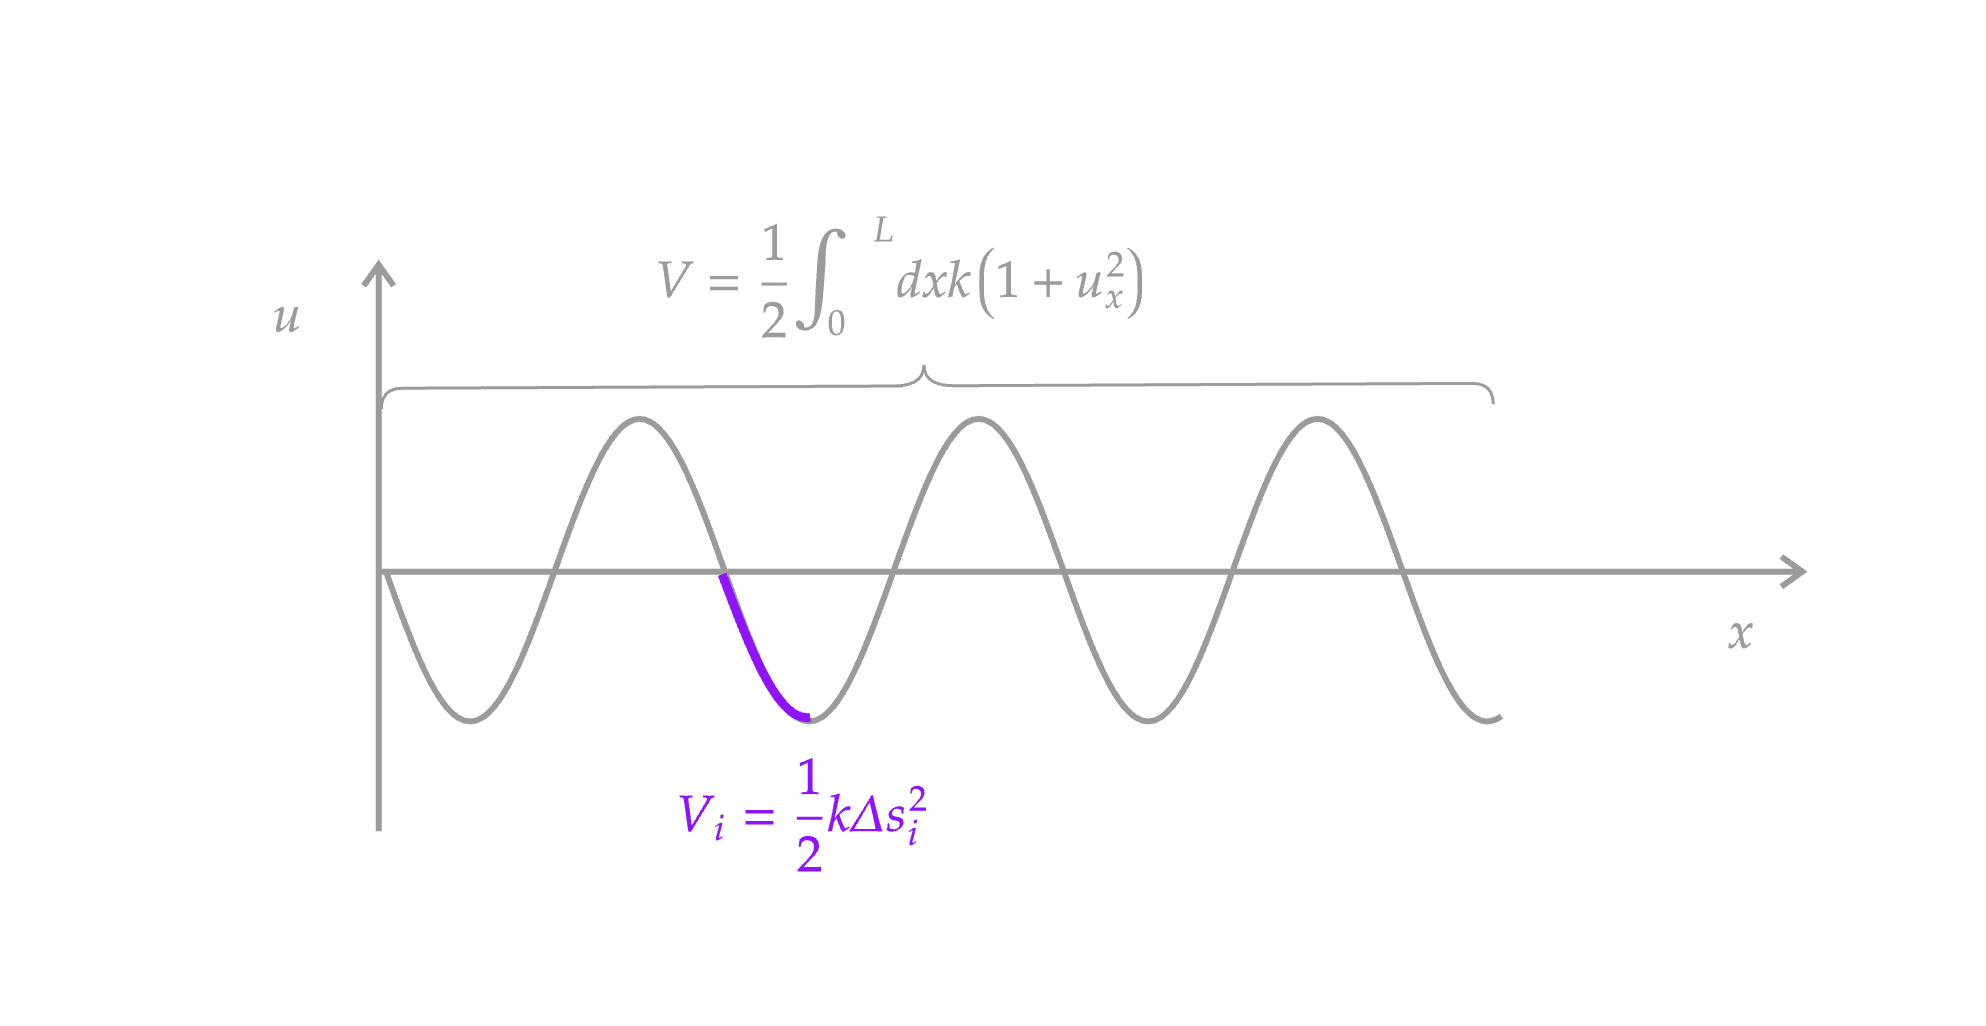
\includegraphics[width=0.7\linewidth]{files/vs-89ee0e6d488b170eecb5d0f3a41cc551.png}
\caption*{The potential energy of a vibrating string.}
\end{figure}

\end{example}We now scrutinize how exactly we optimize (\ref{basicfunctional}).

\subsubsection{Euler-Lagrange Equation}

\begin{theorem}[Euler-Lagrange Equation]$y$ is a stationary point for
\begin{equation}
J[y] = \int_{x_1}^{x_2} f(x,y,y^{(1)},...,y^{(n)})dx
\end{equation}
iff:
\begin{equation}
\boxed{\frac{\partial f}{\partial y} -\frac{d}{dx}\left(\frac{\partial f}{\partial y'}\right)=0}
\end{equation}
The boxed equation is known as the \textbf{Euler-Lagrange Equation}

\end{theorem}\subsubsection{Discretized Euler-Lagrange Equation}

\subsubsection{First Integral}

\begin{definition}[First Integral]Suppose
\begin{equation}
y^{(n)}=f(x,y,y^{(1)},...,y^{(n-1)})
\end{equation}

is an ordinary differential equation of order $n$. We can define an equivalent $n$-dimensional system by letting:
\begin{equation}
y_1 &= y \\
y_2 &= y^{(1)} \\
\vdots \\
y_{n} &= y^{(n-1)}
\end{equation}
Denote by:
\begin{equation}
\frac{dy_i}{dx}=f_i(x,y_1,...,y_n)
\end{equation}
Now suppose $f$ is:

\begin{enumerate}
\item Continous about $x,y_1,...,y_n$
\item Continuously differentialbe about $y_1,...,y_n$
\end{enumerate}

Define  the \textit{first integral} of the $n^{\text{th}}$-order problem to be a function $I=I(x,y_1,...,y_n)$ that also satisfies the above two requirements , and furthermore has the definitive property:
\begin{equation}
I(x,y_1,...,y_n)=\text{Constant}
\end{equation}
along solution curves $\Gamma=(y_1(x),y_2(x),...,y_n(x))$ with the constant determined by the solution curve.

\end{definition}We are confronted by the higher-order ordinary differential equation:
\begin{equation}
\label{ele}
\frac{\partial f}{\partial y} -\frac{d}{dx}\left( \frac{\partial f}{\partial y'}\right)=0
\end{equation}
The compute the first integral of this equation is to rewrite the above to obtain an equation of the form:
\begin{equation}
\frac{d}{dt}I(x,y,y',...)=0
\end{equation}
The strategy is to compute the difference between (\ref{ele}) and the exact differential:
\begin{equation}
\frac{df}{dx}=\frac{\partial f}{\partial x} + \sum_{j\geq 0}\frac{\partial f}{\partial y^{(j)}}\frac{dy^{(j)}}{dx}=\frac{\partial f}{\partial x} +\frac{\partial f}{\partial y}\frac{dy}{dx}+\frac{\partial f}{\partial y^{(1)}}\frac{dy^{(1)}}{dx}+\cdots
\end{equation}
If we multiply (\ref{ele}) by $y'$ and subtract the two equations we get:

\begin{equation}
\frac{df}{dx}-y'\left\{\frac{\partial f}{\partial y} - \frac{d}{dx}\left( \frac{\partial f}{\partial y'}\right)\right\} =\frac{\partial f}{\partial x} + \textcolor{cyan}{y''\frac{\partial f}{\partial y'}+ y'\frac{d}{dx}\left( \frac{\partial f}{\partial y'}\right)}-\sum_{j\geq 2}\frac{\partial f}{\partial y^{(j)}}\frac{dy^{(j)}}{dx}
\end{equation}

\begin{framed}
\textbf{The particular form that allows easy first integral}\\
If we assume $f$ is only dependent on $y,y'$, the above becomes $f(y,y')$, then
\begin{equation}
\sum_{j\geq 2}\frac{\partial f}{\partial y^{(j)}}\frac{dy^{(j)}}{dx} &= 0\\ 
\frac{\partial f}{\partial x} &=0
\end{equation}
\end{framed}

Now:
\begin{equation}
\frac{df}{dx}-\underbrace{y'\left\{\frac{\partial f}{\partial y} - \frac{d}{dx}\left( \frac{\partial f}{\partial y'}\right)\right\}}_{0}&= \frac{d}{dx}\left(y'\frac{\partial f}{\partial y'}\right)
\end{equation}
Hence:
\begin{equation}
\frac{d}{dx}\left(f-y'\frac{\partial f}{\partial y'}\right)=0
\end{equation}
We have sucesfully obtained the first inetgral:
\begin{equation}
I(y,y)=f-y'\frac{\partial f}{\partial y'}
\end{equation}

\subsubsection{Exercises}

\paragraph{Euler-Lagrange Equation for Multiple Independent Variables}

\textbf{Prove} that:

\begin{theorem}[Euler-Lagrange Equation]Consider the functional
\begin{equation}
J[y]=\int f(x_1,x_2,...,x_n,y_{x_1},y_{x_2},...,y_{x_n})d\mathbf{x}
\end{equation}
Show that the stationary is acheived iff:
\begin{equation}
\frac{\partial f}{\partial y} - \sum_{i}\frac{d}{dx}\left(\frac{\partial f}{\partial y_{x_i}}\right)
\end{equation}

\end{theorem}
\bigskip
\centerline{\rule{13cm}{0.4pt}}
\bigskip

\paragraph{Fermat's Principle \footnote{From Dr. P.Draper's homework problems for PHYS 508(\textit{Mathematical Physics I}) at UIUC.}}

\begin{framed}
\textbf{Fermat's Principle}\\
The path taken by a ray of light between any two point makes stationary the travel time between those points.
\end{framed}

We also define:

\begin{definition}[Refractive Index]A medium is characterized by the speed of light traveling through. Specifically, the refractive index is defined by $n=\frac{c}{\text{speed of light traveling in the medium}}$

\end{definition}\begin{framed}
\textbf{\textbf{Problem 1} Light Propagtes in Straight Line in Homogenous Media}\\
\begin{enumerate}
\item \textbf{Show that light propagates along a stragiht line in homogenous media.}
\end{enumerate}
\end{framed}

\begin{framed}
\textbf{\textit{Solution}}\\
Since $n$ is independent of position in homogenous media, make stationary the travel time is equivalent to make stationary the length of the path taken. Now the problem is equivalent to optimizing:
\begin{equation}
\int_{x_1}^{x_2} \sqrt{1+y'^2}dx
\end{equation}
Note:
\begin{equation}
f_y = 0 \quad f_y' = \frac{y'}{\sqrt{1+y'^2}}
\end{equation}
The Euler-Lagrange equation is, therefore:
\begin{equation}
\frac{}{}
    \frac{d}{dx}\left[ \frac{y'}{\sqrt{1+y'^2}}\right] &= 0 \\
    \frac{y'}{\sqrt{1+y'^2}} &= C_1
\end{equation}
Note the L.H.S is a non-constant function of $y'$, hence:
\begin{equation}
y'= C_2 \Longrightarrow y=C_2x+C_3
\end{equation}
\end{framed}

\begin{framed}
\textbf{\textbf{Problem 2} Snell's Law}\\
Consider the propagation of light from a flat slab of glass of refractive index $n_1$ into to
another with refractive index $n_2$. By examining paths that need not be differentiable
at the flat interface, establish Snell's law:
\begin{equation}
n_1\sin(\theta_1) = n_2\sin(\theta_2)
\end{equation}
\end{framed}

\begin{framed}
\textbf{\textit{Solution}}\\
We consider the first point at $(x_1, 0)$, the second point at $(x_2,y_2)$ where $x_1<0<x_2$. The time taken is hence:
\begin{equation}
\int_{x_1}^{x_2} \frac{1}{v(x)}\sqrt{1+y'^2}dx
\end{equation}
where:
\begin{equation}
v(x)=
\begin{cases}
    c/n_1 &\text{if } x<0 \\
    c/n_2 &\text{if } x>0
\end{cases}
\end{equation}
The Euler-Lagrange equation is:
\begin{equation}
0 + \frac{d}{dx}\left( \frac{y'}{v(x)\sqrt{1+y'^2}} \right)=0
\end{equation}
Hence:
\begin{equation}
\frac{y'}{v(x)\sqrt{1+y'^2}} =C
\end{equation}
For $x<0$, we have:
\begin{equation}
\frac{1}{v(x)}\frac{y'}{\sqrt{1+y'^2}} = \frac{n_1}{c}\sin(\theta_1) = C_1
\end{equation}
For $x>0$, we have:
\begin{equation}
\frac{1}{v(x)}\frac{y'}{\sqrt{1+y'^2}} = \frac{n_2}{c}\sin(\theta_2) = C_2
\end{equation}
Hence:
\begin{equation}
n_1\sin(\theta_1)=n_2\sin(\theta_2)
\end{equation}
\textbf{Question:} If we flip the axis we would get $n_1\cos\theta_1=n_2\cos\theta_2$, why is that wrong?
\end{framed}

\begin{framed}
\textbf{\textbf{Problem 3} General Snell's law}\\
A planar light ray propagates in an layered medium with refractive index $n(x)$. Use Fermat's principle to establish a generalized Snell's law:
\begin{equation}
n(x)\sin(\psi(x))=\text{constant}
\end{equation}
by finding the equation for stationary paths for
\begin{equation}
F_1=\int n(x)\sqrt{1+y'^2}dx
\end{equation}
(Here the prime denotes differentiation with respect to x.) Repeat this exercise with $x,y$ swapped by finding a similar equation for the stationary paths of
\begin{equation}
F_2=\int n(y)\sqrt{1+y'^2}dx
\end{equation}
By using suitable definitions of the angle of incidence $\psi$, in each case show that the two formulations of the problem of a layered medium give physically equivalent answers.
(In the second formulation you will find it easiest to use the first integral.)
\end{framed}

\paragraph{Drums and Membranes \footnote{From Dr. P.Draper's homework problems for PHYS 508(\textit{Mathematical Physics I}) at UIUC.}}

The shape of a distorted drumskin is described by the
function $h(x, y)$, which gives the height to which the point $(x, y)$ of the flat undistorted drumskin is displaced.

\begin{framed}
\textbf{\textbf{Problem 1} Area of distorted drumskin}\\
Show that the area of the distorted drumskin is equal to
\begin{equation}
A[h] = \int dxdy \sqrt{1 + \partial_x h^2 + \partial_y h^2}
\end{equation}
\end{framed}

\begin{framed}
\textbf{\textit{Solution}}\\
Consider the area differntial $dA=ds_x ds_y$ where $ds_x=\sqrt{1+\partial_x h^2}dx$ and $ds_y=\sqrt{1+\partial_y h^2}dy$ hence
\begin{equation}
dA=\sqrt{1+\partial_x h^2 + \partial_y h^2 + (\partial_x h\partial_y h)^2}dxdy
\end{equation}
since $\partial_x h\partial_y h\in \mathcal{O}(d\rho^2)$ where $d\rho = \sqrt{dx^2 + dy^2}$ we can drop it. As desired.
\end{framed}

\begin{framed}
\textbf{Area for small distortion}\\
Show that for small distortions, the area reduces to
\begin{equation}
\label{afsd}
   A[h]=\frac{1}{2}\int dxdy |\nabla h|^2 + \text{constant}
\end{equation}
\end{framed}

\begin{framed}
\textbf{\textit{Solution}}\\
Recall the generalized binomial theorem:
\begin{equation}
(1+x)^{\alpha}=1+\alpha x + \frac{\alpha(\alpha-1)}{2!}x^2+\cdots + \frac{\alpha(\alpha-1)...(\alpha-n+1)}{n!}x^n + \cdots
\end{equation}
for $|x|<1$.
As a result:
\begin{equation}
(1+x)^{1/2}=1+\frac12 x + \mathcal{O}(x^2)
\end{equation}
Assume a small perturbation, in particular, assume $|\nabla h|^2 \ll 1$, then
\begin{equation}
\sqrt{1+|\nabla h|^2} = 1 + \frac12 |\nabla h|^2 +  \mathcal{O}(|\nabla h|^4)
\end{equation}
As a result,
\begin{equation}
A[h]=\frac12 \int dxdy |\nabla h|^2 + \underbrace{\int dxdy}_{\text{constant}}
\end{equation}
\end{framed}

\begin{framed}
\textbf{\textbf{Problem 3}}\\
Show that if $h$ satisfies the two-dimensional Laplace equation then $A$ is stationary with
respect to variations that vanish at the boundary.
\end{framed}

\begin{framed}
\textbf{\textit{Solution}}\\
We need that the Euler-Lagrange equation for (\ref{afsd}) is equivlanet to the tow-dimensional Laplace equation. That is simple: let $f(x,y,h, h_x,h_y)=h_x^2 + h_y^2$,
\begin{equation}
\frac{\partial f}{\partial h} + \frac{d}{dx}\left(\frac{\partial f}{\partial h_x}\right) + \frac{d}{dy}\left(\frac{\partial f}{\partial h_y}\right) &= 0 \\
 0 + 2\left(\frac{dh_x}{dx} +  \frac{dh_x}{dx}\right) &= 0\\
 \nabla^2 h &=0
\end{equation}
\end{framed}

\begin{framed}
\textbf{\textbf{Problem 4}}\\
Suppose the drumskin has mass $\rho_0$ per unit area, and surface tension $T$. Write down
the Lagrangian controlling the motion of the drumskin and derive the equation of
motion that follows from it.
\end{framed}

\begin{framed}
\textbf{\textit{Solution}}\\
The kinetic term is given by:
\begin{equation}
T=\frac12 \int_{\Omega} dxdy \rho_0h_t^2
\end{equation}

The potential term is: \footnote{The key to solve this problem is actually to realize that surface tension has the dimension $[F]/[L]=[E]/[L]^2$, in otherword, surface tension is precisely the perunit potential energy due to ``stretching''/``distorsion'' by construction.}
\begin{equation}
V=\int_{\Omega} dxdy T|\nabla h|^2
\end{equation}

Hence the lagrangian is:
\begin{equation}
L &= T-V \\
&= \int_{\Omega} dxdy \left\{\frac12 \rho_0h_t^2 - T|\nabla h|^2 \right\}
\end{equation}

Computing the various derivatives:
\begin{equation}
\frac{\partial L}{\partial h}=0 \quad \frac{\partial L}{\partial h_t}=\rho_0 h_t \quad \frac{\partial L}{\partial h_x}=-2Th_{x} \quad \frac{\partial L}{\partial h_y}=-2Th_{y}
\end{equation}
\end{framed}